\chapter{Analyse}
\label{ch:Analysis}



\section{Übersicht und Kennzahlen}
\label{sec:overview-numbers}
Als erstes soll die Art des Netzwerkes analysiert werden. Der Begriff \guillemotleft Hub\guillemotright wird sehr
häufig im Zusammenhang mit Luftfahrt und Flughäfen verwendet.
Deshalb wird auch erwartet, dass das Netzwerk ein natürliches Netzwerk bildet.
Zufällige Netzwerke haben eine gleichmässige Gradverteilung während die Verteilung bei natürlichen Netzwerken einem
Potenzgesetz folgt.
Das Histogramm der Knotengrade deutet sehr stark auf eine exponentielle Verteilung hin (siehe Abb. \ref{fig:degreeHistogram}).

\begin{figure}
    \centering
    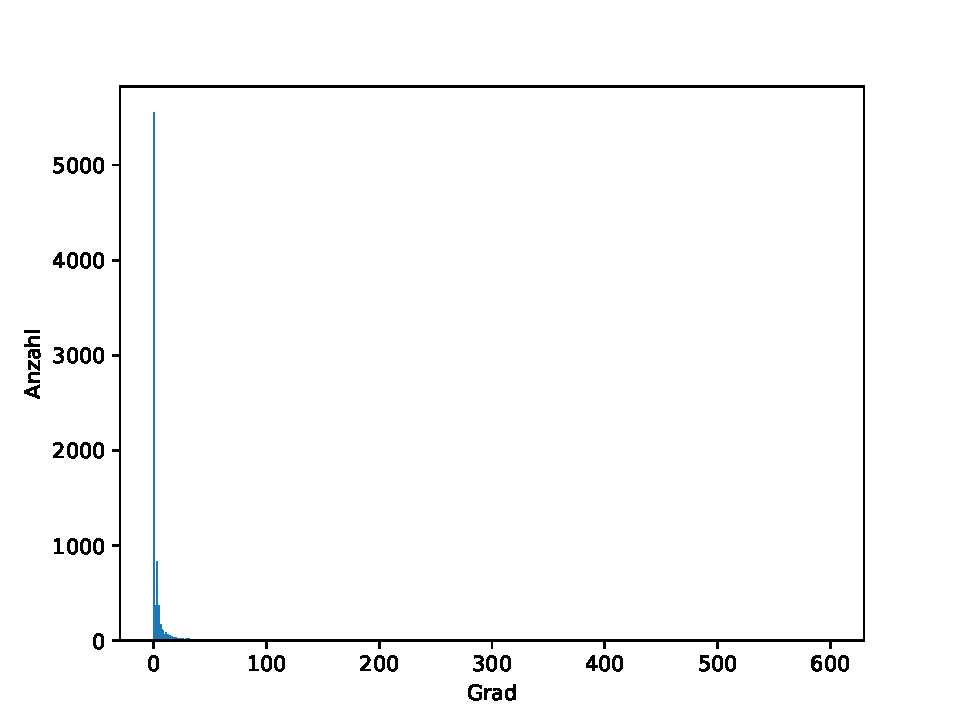
\includegraphics[width=0.75\linewidth]{images/degree-histogram.pdf}
    \caption{Caption}
    \label{fig:degreeHistogram}
\end{figure}

\subsection{Kennzahlen}

\langle k\rangle = 5.455
Diameter: 10
\gamma

\subsection{Durchmesser des Netzwerks}
10



\section{Erste Forschungsfragen}
\label{sub:scientific-questions}

\begin{enumerate}
    \item Welches sind die wichtigsten Flughäfen?
    \item Welches ist der Zeitgünstigste Weg, um von Zürich nach Zürich einmal um die Welt zu fliegen?
    \item Wie ist die Beschaffenheit des globalen Flughafennetzwerkes im Bezug auf die Robustheit?
\end{enumerate}

\subsection{Ausarbeitung}
\label{subsec:scientific-question-analysis}


\subsubsection{Welches sind die wichtigsten Flughäfen?}
Begründung: Wichtig für die Funktionstüchtigkeit des Netzwerks

\subsubsection{Welches ist der Zeitgünstigste Weg, um von Zürich nach Zürich einmal um die Welt zu fliegen?}
Begründung: Aviatik hat jeden Punkt auf der Erde in wenigen Stunden erreichbar gemacht. Aber wie lange dauert eine komplette Erdumrundung konkret?

\subsubsection{Wie ist die Beschaffenheit des globalen Flughafennetzwerkes im Bezug auf die Robustheit?}
Begründung: Im Flugnetz finden täglich bis zu 200000 Flugbewegungen statt \footnote{http://www.reisereporter.de/artikel/4533-rekord-tag-luftfahrtgeschichte-flugzeuge-und-fluege-pro-tag-weltweit-flug-tracker-flightradar-misst-verkehrsreichsten-tag}.
Für diese enorme Zahl finden erstaunlich wenige Störungen und Ausfälle statt.
Aber wie gut ist das Netzwerk aufgebaut?
Wieviele Flughäfen müssten ausfallen, damit das Gesamtnetz in einzelne isolierte Unternetze zerfällt und damit der weltweite Luftverkehr zum erliegen kommt?
Robustheit, relevanz? Heisst: Wie lange hängen alle noch aktiven Flughäfen zusammen?

Random Failuers: f_c = 1 - \frac{1}{\frac{\langle k^{2}\rangle}{\langle k\rangle} - 1} = 0.775533


\section{Literatur-Recherche}
\label{subsec:literature-research}

Robustheit

\guillemotleft Worldwide aviation network vulnerability analysis: a complex network approach \guillemotright
https://link-springer-com.proxy2.biblio.supsi.ch/content/pdf/10.1007%2Fs40844-015-0025-y.pdf

Als besseres Mass für die Robustheit gilt die die Auswirkung auf die Effizienz, wenn bestimmte Flughäfen aussteigen.


Verspätungen

\guillemotleft Systemic delay propagation in the US airport network \guillemotright
https://www.nature.com/articles/srep01159
https://www.nzz.ch/wirtschaft/wieso-in-europa-viel-zu-viele-fluege-verspaetet-sind-ld.1410842

Sagt düstere Zukunft voraus in nächster Dekade, da System möglicherweise überlastet.
Hauptursache für Verbreitung von Verspätungen sind Anschlussflüge.
Verspätungen ballen sich meist in Clustern.



\subsection{Weitere Forschungsfragen}
\begin{enumerate}
    \item Wie wichtig sind ausgewählte Flughäfen für die Effizienz des Gesamtnetzwerkes?
    \item Wie empfindlich ist das europäische Netzwerk auf Verspätungen?
    \item Wie wirkt sicht ein Zuwachs von x \% auf die Empfindlichkeit aus?
\end{enumerate}

\subsubsection{Wie wichtig sind ausgewählte Flughäfen für die Effizienz des Gesamtnetzwerkes?}
Begründung: Ist das Vorhandensein eines Flughafens Fluch oder Segen? Wäre die Effizienz des Gesamtnetzerks rebuster, wenn der Flughafen gar nicht existieren würde?

\subsubsection{}
